\documentclass[a4paper,12pt]{article} % тип документа

% report, book

%  Рисунки
\usepackage{graphicx}
\usepackage{wrapfig}

%  Русский язык

\usepackage[T2A]{fontenc}			% кодировка
\usepackage[utf8]{inputenc}			% кодировка исходного текста
\usepackage[english,russian,]{babel}	% локализация и переносы
\usepackage{xymtex}
\usepackage{amsmath,amsfonts,amssymb,amsthm,mathtools} 
\usepackage{setspace,amsmath}
\usepackage{wasysym}
\usepackage[left=1.27cm,right=1.27cm,top=1.27cm,bottom=2cm, footskip=10mm]{geometry}% настройки полей документа
\RequirePackage{caption2}
\usepackage{float}
\usepackage{ragged2e}
\justifying
%\usepackage[usenames]{color}
\usepackage{icomma} % "Умная" запятая: $0,2$~-— число, $0, 2$~-— перечисление 
\usepackage{upgreek} 
%\usepackage[14pt]{extsizes} % для того чтобы задать нестандартный 14-ый размер шрифта

\usepackage{gensymb}
\usepackage{esint}
\usepackage{gnuplottex} 


% running titles 
\usepackage{fancybox}
\usepackage{fancyhdr}

% for diff running titles on pages with diff parity
\usepackage{ifthen}
\usepackage{pdfpages}
\usepackage[strict]{changepage}

%%% Оформление 
\usepackage{indentfirst} % Красная строка 
\setlength{\parskip}{0.3cm} % отступы между абзацами 

%%% Теоремы 
\theoremstyle{plain} % Это стиль по умолчанию, его можно не переопределять. 
\newtheorem{theorem}{Теорема}[section] 
\newtheorem{proposition}[theorem]{Утверждение} 

\theoremstyle{definition} % "Определение" 
\newtheorem{definition}{Определение}[section] 
\newtheorem{corollary}{Следствие}[theorem] 
\newtheorem{problem}{Задача}[section] 

\theoremstyle{remark} % "Примечание" 
\newtheorem*{nonum}{Решение} 
\newtheorem{zamech}{Замечание}[theorem] 

% Ссылки
\usepackage{xcolor}
\usepackage{color} % подключить пакет color
% выбрать цвета
\definecolor{BlueGreen}{RGB}{49,152,255}
\definecolor{Violet}{RGB}{120,80,120}
% назначить цвета при подключении hyperref
\usepackage[unicode, colorlinks, urlcolor=blue, linkcolor=blue, pagecolor=blue, citecolor=blue]{hyperref} %синие ссылки
%\usepackage[unicode, colorlinks, urlcolor=black, linkcolor=black, pagecolor=black, citecolor=black]{hyperref} % для печати (отключить верхний!)
%\mathtoolsset{showonlyrefs=true} % Показывать номера только у тех формул, на которые есть \eqref{} в~тексте.

% Цвета для гиперссылок
\definecolor{linkcolor}{HTML}{799B03} % цвет ссылок
\definecolor{urlcolor}{HTML}{799B03} % цвет гиперссылок
 
\hypersetup{pdfstartview=FitH,  linkcolor=linkcolor,urlcolor=urlcolor, colorlinks=true}

% for lab number change in all doc
\newcommand{\labnum}{
	2.4.1
}

% page style setup (for running titles)
\fancypagestyle{plain}{ %
	\fancyhf{} % remove everything
	
	 % lines parameters
	\renewcommand{\headrulewidth}{0pt}
	\renewcommand{\footrulewidth}{0pt}
	
	% running titles contents
	\fancyfoot[L]{\ifthenelse{\isodd{\thepage}}{Работа \labnum}{\thepage}}
	\fancyfoot[R]{\ifthenelse{\isodd{\thepage}}{\thepage}{Работа \labnum}}
}

% choosing page style with our running titles
\pagestyle{plain}

\usepackage[left=1.27cm,right=1.27cm,top=1.27cm,bottom=2cm]{geometry}
\begin{document} % начало документа
 
\begin{center}
\hfill \break

\small{\textbf{«МОСКОВСКИЙ ФИЗИКО-ТЕХНИЧЕСКИЙ ИНСТИТУТ (НАЦИОНАЛЬНЫЙ ИССЛЕДОВАТЕЛЬСКИЙ УНИВЕРСИТЕТ)»}}\\
\hfill \break
\hfill \break
\Large\textbf{{Лабораторная работа 2.4.1}}\\
\Large{Определение теплоты испарения жидкости}\\

\text{Матренин Василий Б01-006 ФРКТ}\\
\end{center}

\vspace{2cm}

\noindent\textbf{Цель работы:} 1) измерение давления насыщенного пара жидкости при разной температуре; 2) вычисление по полученным данным теплоты испарения с помощью уравнения Клапейрона–Клаузиуса.

\noindent\textbf{В работе используются:} термостат; герметический сосуд, заполненный исследуемой жидкостью; отсчетный микроскоп.

\section*{Теоретическая справка}
Испарением называется переход вещества из жидкого в газообразное состояние. Оно происходит на свободной поверхности жидкости.
При испарении с поверхности вылетают молекулы, образуя над ней пар. Для выхода из жидкости молекулы должны преодолеть силы молекулярного сцепления. Кроме того, при испарении совершается работа против внешнего давления P, поскольку объем жидкости меньше объема пара. Не все молекулы жидкости способны совершить эту работу, а только те из них, которые обладают достаточной кинетической энергией. Поэтому переход части молекул в пар приводит
к обеднению жидкости быстрыми молекулами, т. е. к ее охлаждению. Чтобы испарение проходило без изменения температуры,
к жидкости нужно подводить тепло. Количество теплоты, необходимое для изотермического испарения одного моля жидкости при внешнем давлении, равном упругости ее насыщенных паров, называется молярной теплотой испарения (парообразования).

Теплоту парообразования жидкостей можно измерить непосредственно при помощи
калориметра. Такой метод, однако, не позволяет получить точных результатов из-за неконтролируемых потерь тепла,
которые трудно сделать малыми. В настоящей работе для определения теплоты испарения применен
косвенный метод, основанный на уравнении Клапейрона–Клаузиуса:
\begin{equation}
\dfrac{dP}{dT}=\dfrac{L}{T(V_2-V_1)}.
\end{equation}
Здесь $P$-- давление насыщенного пара жидкости при температуре $T, ~T$-- абсолютная температура жидкости и пара,
$L$-- теплота испарения жидкости,
$V_2$ -- объем пара,
$V_1$ -- объем жидкости. Найдя из
опыта $\frac{dP}{dT},~T,~ V_2$ и
$V_1$, можно определить $L$ путем расчета. Величины $L,~ V_2$ и
$V_1$ в формуле (1) должны относиться к одному и тому же количеству вещества; мы будем относить их
к одному молю.

В нашем приборе измерения производятся при давлениях ниже атмосферного.
В этом случае задача существенно упрощается.
В таблице для ряда жидкостей приведены: температура, при которой давление насыщенных паров равно атмосферному, величины $V_2$ и $V_1$, входящие в (1), а также константы $a$ и $b$ в уравнении Ван-дер-Ваальса.

Из таблицы видно, что $V_1$ не превосходит 0,5\% от $V_2$. При нашей точности опытов величиной $V_1$ в (1) можно пренебречь.

Обратимся теперь к $V_2$, которое в дальнейшем будем обозначать просто $V$ . Объем $V$ связан с давлением
и температурой уравнением Ван-дер-Ваальса:
\begin{equation}
\left(P-\dfrac{a}{V^2}\right)(V-b)=RT.
\end{equation}

Из рассмотрения таблицы следует, что b одного порядка с $V_1$. В уравнении Ван-дер-Ваальса величиной $b$ следует пренебречь. Пренебрежение членом $\frac{a}{V^2}$ по сравнению с $P$ вносит ошибку менее 3\%. При давлении ниже атмосферного ошибки становятся еще меньше.
Таким образом, при давлениях ниже атмосферного уравнение Ван-дер-Ваальса для насыщенного пара мало отличается от уравнения Клапейрона.
Положим поэтому
\begin{equation}
V=\dfrac{RT}{P}.
\end{equation}
Подставляя (3) в (1), пренебрегая
$V_1$ и разрешая уравнение относительно $L$, найдем

\begin{equation}
L=\dfrac{RT^2}{P}\dfrac{dP}{dT}=-R\dfrac{d(\ln P)}{d(1/T)}.
\end{equation}

В нашем опыте температура жидкости измеряется термометром, давление пара определяется при помощи манометра,
а производные $\frac{dP}{dT}$ или $\frac{d(\ln P)}{d(1/T)}$ находятся графически как угловой коэффициент касательной к
кривой $P(T)$ или соответственно к кривой, у которой по оси абсцисс отложено $\frac{1}{T}$, а по оси ординат $\ln P$.

\textbf{Экспериментальная
установка.} Схема установки изображена на рисунке 1.
Наполненный водой резервуар 1 играет роль термостата. Нагревание термостата производится спиралью 2, подогреваемой электрическим током. Для охлаждения воды в термостате через змеевик 3. 
\begin{wrapfigure}{r}{4.5cm}
	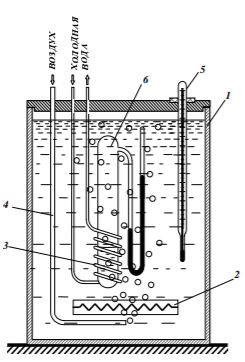
\includegraphics[scale=1]{im1}
	\caption{ {\small Схема установки для определения теплоты испарения}}
\end{wrapfigure}
пропускается водопроводная вода. Вода в термостате перемешивается воздухом,
поступающим через трубку 4.
Температура воды измеряется термометром 5.
В термостат погружен запаянный прибор 6 с исследуемой жидкостью. Над ней находится насыщенный пар (перед заполнением прибора воздух из него был откачан).
Давление насыщенного пара определяется по ртутному манометру, соединенному с исследуемым объемом. Отсчет показаний манометра
производится при помощи микроскопа.

На рисунке 2 приведена более полная схема такой
же установки, но с использованием современного термостата.
Установка включает термостат A, экспериментальный прибор B и отсчетный микроскоп C. На рисунке 2 работы 2.2.6 приведен внешний вид термостата. Там
же описан порядок работы с ним.
Экспериментальный прибор
B представляет собой емкость 12, заполненную водой.
В нее погружен запаянный прибор 13 с исследуемой жидкостью 14. Перед заполнением исследуемой жидкости воздух
из запаянного прибора был удален, так что над жидкостью находится только её насыщенный пар. Давление пара определяется по ртутному
манометру 15, соединенному с ёмкостью 13. Численная величина давления измеряется по разности показаний отсчетного микроскопа 16,
настраиваемого последовательно на нижний и верхний уровни столбик
а ртути манометра. Показания микроскопа снимаются по шкале 17.

\begin{figure}[H]
	\centering
	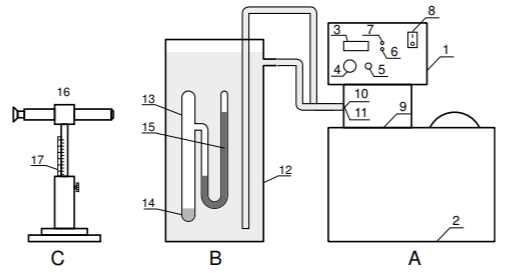
\includegraphics[scale=1]{im2}
	\caption{Схема установки для определения теплоты испарения}
\end{figure}

Описание прибора указывает на второе важное преимущество
предложенного косвенного метода измерения $L$ перед прямым. При
непосредственном измерении теплоты испарения опыты нужно производить при неизменном давлении,
и прибор не может быть запаян. При этом невозможно обеспечить такую чистоту
и неизменность экспериментальных условий,
как при нашей постановке опыта.

Описываемый прибор обладает важным недостатком: термометр
определяет температуру термостата,
а не исследуемой жидкости (или ее пара). Эти температуры близки друг
к другу лишь в том случае, если нагревание происходит достаточно медленно. Убедиться в том,
что темп нагревания не является слишком быстрым, можно, сравнивая результаты, полученные при нагревании
и при остывании прибора. Такое сравнение необходимо сделать. Для ориентировки укажем,
что температуру воды в калориметре следует менять не быстрее, чем
на $\rm 1^{\circ}C$ в течение 1–3 минут.

\section*{Обработка результатов}

Построим таблицу при повышении температуры.
\begin{table}[H]
\begin{center}
\begin{tabular}{|c|c|c|c|c|c|c|c|}
\hline
\multicolumn{8}{|c|}{\textbf{Таблица 1. Температурная зависимость давления при нагревании}}                                                                                   \\ \hline
\textbf{N} & \textbf{T, K} & \textbf{$h_{min}$, мм} & \textbf{$h_{max}$, мм} & \textbf{$\delta_{h}$, мм} & \textbf{P, Па} & \textbf{1/T * $10^{3}$, $K ^ {-1}$} & \textbf{lnp} \\ \hline
1          & 293,15        & 81,2                   & 98,1                   & 16,9                      & 2 254,73       & 3,41                                & 7,72         \\ \hline
2          & 294,15        & 80,8                   & 98,7                   & 17,9                      & 2 388,15       & 3,40                                & 7,78         \\ \hline
3          & 295,15        & 80                     & 99,3                   & 19,3                      & 2 574,93       & 3,39                                & 7,85         \\ \hline
4          & 296,15        & 79,4                   & 100                    & 20,6                      & 2 748,37       & 3,38                                & 7,92         \\ \hline
5          & 297,15        & 78,7                   & 100,7                  & 22                        & 2 935,15       & 3,37                                & 7,98         \\ \hline
6          & 298,15        & 78                     & 101,3                  & 23,3                      & 3 108,59       & 3,35                                & 8,04         \\ \hline
7          & 299,15        & 77,5                   & 102                    & 24,5                      & 3 268,69       & 3,34                                & 8,09         \\ \hline
8          & 300,15        & 76,6                   & 102,9                  & 26,3                      & 3 508,84       & 3,33                                & 8,16         \\ \hline
9          & 301,15        & 75,8                   & 103,4                  & 27,6                      & 3 682,28       & 3,32                                & 8,21         \\ \hline
10         & 302,15        & 75                     & 104,4                  & 29,4                      & 3 922,43       & 3,31                                & 8,27         \\ \hline
11         & 303,15        & 74,1                   & 105,2                  & 31,1                      & 4 149,24       & 3,30                                & 8,33         \\ \hline
12         & 304,15        & 73,5                   & 106,3                  & 32,8                      & 4 376,04       & 3,29                                & 8,38         \\ \hline
13         & 305,15        & 72,5                   & 107,2                  & 34,7                      & 4 629,54       & 3,28                                & 8,44         \\ \hline
14         & 306,15        & 71,6                   & 108,2                  & 36,6                      & 4 883,03       & 3,27                                & 8,49         \\ \hline
15         & 307,15        & 70,6                   & 109,2                  & 38,6                      & 5 149,86       & 3,26                                & 8,55         \\ \hline
16         & 308,15        & 69,5                   & 110,3                  & 40,8                      & 5 443,37       & 3,25                                & 8,60         \\ \hline
17         & 309,15        & 68,3                   & 111,7                  & 43,4                      & 5 790,25       & 3,23                                & 8,66         \\ \hline
18         & 310,15        & 67,2                   & 112,8                  & 45,6                      & 6 083,77       & 3,22                                & 8,71         \\ \hline
19         & 311,15        & 66                     & 114,1                  & 48,1                      & 6 417,31       & 3,21                                & 8,77         \\ \hline
20         & 312,15        & 64,7                   & 115,5                  & 50,8                      & 6 777,53       & 3,20                                & 8,82         \\ \hline
21         & 313,15        & 63,3                   & 116,8                  & 53,5                      & 7 137,76       & 3,00                                & 8,87         \\ \hline
\end{tabular}
\end{center}
\end{table}


\newpage
Построим таблицу при понижении температуры.
\begin{table}[H]
\begin{center}
\begin{tabular}{|c|c|c|c|c|c|c|c|}
\hline
\multicolumn{8}{|c|}{\textbf{Таблица 2. Температурная зависимость давления при охлаждении}}                                                                                   \\ \hline
\textbf{N} & \textbf{T, K} & \textbf{$h_{min}$, мм} & \textbf{$h_{max}$, мм} & \textbf{$\delta_{h}$, мм} & \textbf{P, Па} & \textbf{1/T * $10^{3}$, $K ^ {-1}$} & \textbf{lnp} \\ \hline
1          & 313,15        & 63,4                   & 116,9                  & 53,5                      & 7 137,76       & 3,19                                & 8,87         \\ \hline
2          & 312,15        & 64,1                   & 115,5                  & 51,4                      & 6 857,58       & 3,20                                & 8,83         \\ \hline
3          & 311,15        & 65,9                   & 114,5                  & 48,6                      & 6 484,02       & 3,21                                & 8,78         \\ \hline
4          & 310,15        & 66,6                   & 113,1                  & 46,5                      & 6 203,84       & 3,22                                & 8,73         \\ \hline
5          & 309,15        & 68,2                   & 112,2                  & 44                        & 5 870,30       & 3,23                                & 8,68         \\ \hline
6          & 308,15        & 68,8                   & 110,7                  & 41,9                      & 5 590,13       & 3,25                                & 8,63         \\ \hline
7          & 307,15        & 70                     & 109,6                  & 39,6                      & 5 283,27       & 3,26                                & 8,57         \\ \hline
8          & 306,15        & 71,3                   & 108,6                  & 37,3                      & 4 976,42       & 3,27                                & 8,51         \\ \hline
9          & 305,15        & 71,9                   & 107,5                  & 35,6                      & 4 749,61       & 3,28                                & 8,47         \\ \hline
10         & 304,15        & 72,9                   & 106,5                  & 33,6                      & 4 482,78       & 3,29                                & 8,41         \\ \hline
11         & 303,15        & 73,8                   & 105,5                  & 31,7                      & 4 229,29       & 3,30                                & 8,35         \\ \hline
12         & 302,15        & 75                     & 104,5                  & 29,5                      & 3 935,77       & 3,31                                & 8,28         \\ \hline
13         & 301,15        & 75,7                   & 103,7                  & 28                        & 3 735,65       & 3,32                                & 8,23         \\ \hline
14         & 300,15        & 76,6                   & 102,8                  & 26,2                      & 3 495,50       & 3,33                                & 8,16         \\ \hline
15         & 299,15        & 77,2                   & 101,9                  & 24,7                      & 3 295,38       & 3,34                                & 8,10         \\ \hline
16         & 298,15        & 78                     & 101,4                  & 23,4                      & 3 121,93       & 3,35                                & 8,05         \\ \hline
17         & 297,15        & 78,6                   & 100,5                  & 21,9                      & 2 921,81       & 3,37                                & 7,98         \\ \hline
18         & 296,15        & 79,3                   & 100                    & 20,7                      & 2 761,71       & 3,38                                & 7,92         \\ \hline
19         & 295,15        & 79,6                   & 99,3                   & 19,7                      & 2 628,30       & 3,39                                & 7,87         \\ \hline
20         & 294,15        & 80,2                   & 98,8                   & 18,6                      & 2 481,54       & 3,40                                & 7,82         \\ \hline
21         & 293,15        & 80,7                   & 98,2                   & 17,5                      & 2 334,78       & 3,41                                & 7,76         \\ \hline
\end{tabular}
\end{center}
\end{table}

\newpage
Построим график зависимости P от T при нагревании.

\begin{figure}[H]
    \centering
	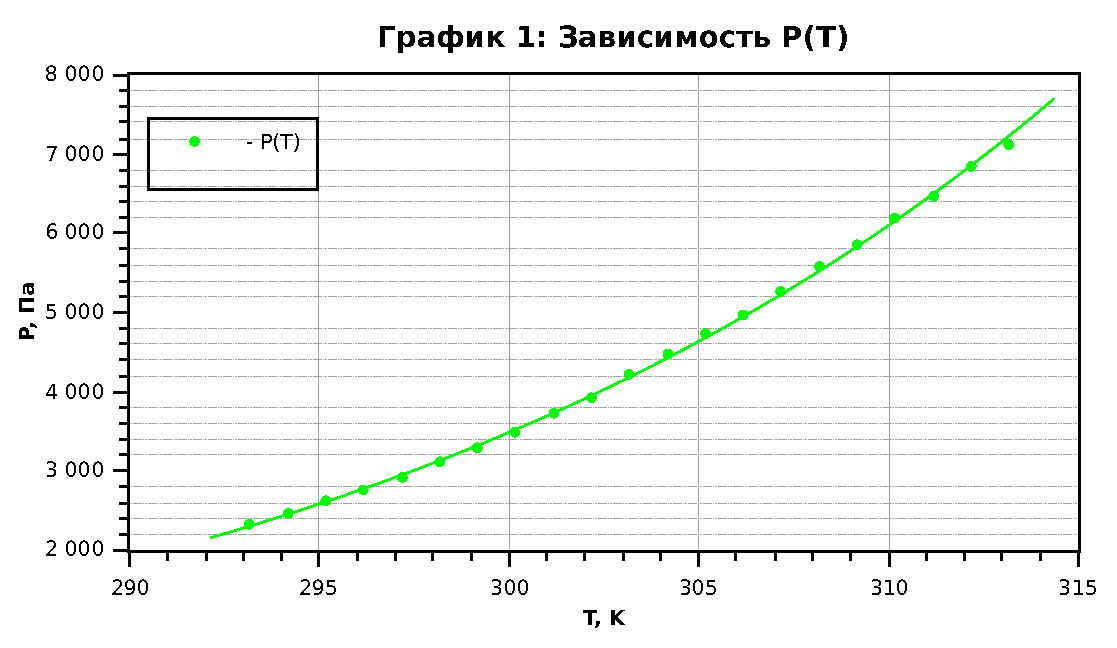
\includegraphics[scale=0.8]{Graph1.pdf}
	%\caption{График зависимости P от T}
\end{figure} 


Рассмотрим уравнение Клапейрона-Клаузиуса:
\[\dfrac{dP}{dT}=\dfrac{L}{T(V_2-V_1)}\approx \dfrac{PL}{RT^2};\]
\[\int \dfrac{dP}{P}=\dfrac{L}{R} \int \dfrac{dT}{T^2};\]
\[\ln(P)=-\dfrac{L}{R}\cdot \dfrac{1}{T}+C;\]
\[P(T)=e^C\cdot e^{-\frac{1}{RT}L}.\]
Найдём среднее значение показателя экспоненты $n$:
%\[\bar{n}=-\frac{0,055+0,052}{2}=-0,0535.\]
\[\bar{n}=-\frac{0,049+0,048}{2}=-0,0485.\]

Тогда получим
\[L=\bar{n}RT\]
Но тогда $L=f(T)$, а значит, $L$ будет разным при различных температурах.

Рассмотрим график зависимости $\ln(P)$ от $\frac{1}{T}$.

\begin{figure}[H]
    \centering
	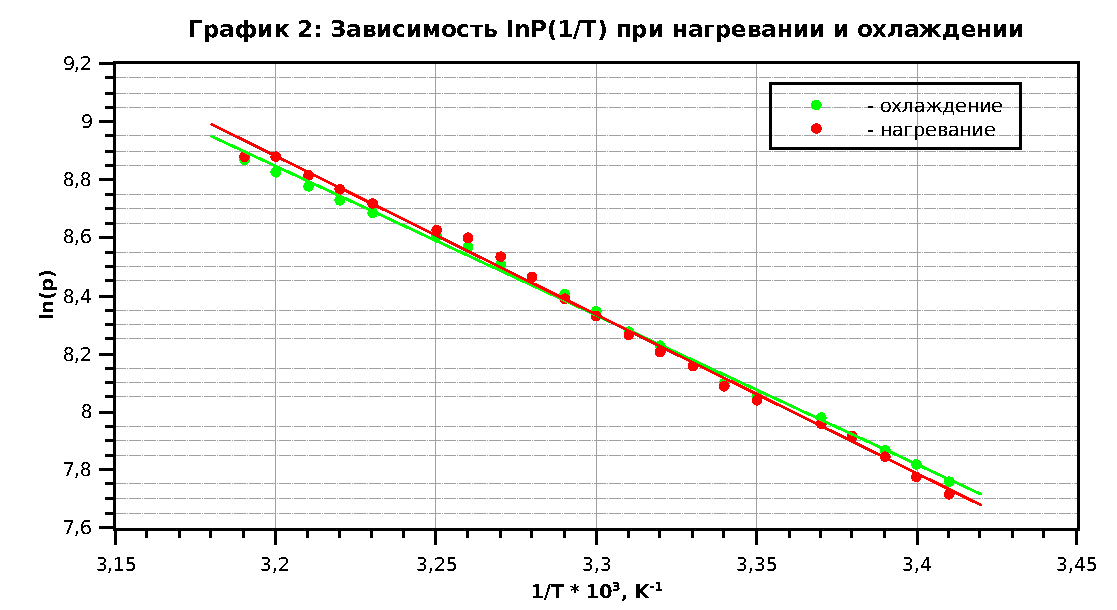
\includegraphics[scale=0.8]{Graph2.pdf}
	%\caption{График зависимости $\ln(P)$ от $\frac{1}{T}$}
\end{figure}

Получим, что коэффциент наклона, $\bar{k}=(k_1+k_2)\div 2\approx-5301,25$.

Тогда по формуле (4) $L=-R\bar{k}=-8,314\cdot(-5301,25)\approx44,075\cdot 10^3~\frac{\text{Дж}}{\text{моль}}$.

Оценим возможную ошибку измерений

\[\left(\dfrac{\sigma_L}{L}\right)^2=\left(\dfrac{\sigma_{k}}{k}\right)^2; \]
\[\sigma_L=L\dfrac{\sigma_{k}}{k}\approx612~\frac{\text{Дж}}{\text{моль}}~~(\sigma= 1,4\%). \]

%\section*{Обсуждение результатов}

В ходе проведённых измерений было получено значение теплоты испарения воды \\
$L=(44,1 \pm 0,6) \cdot 10^3~\frac{\text{Дж}}{\text{моль}}$, что близко к справочному значению $L=40662~\frac{\text{Дж}}{\text{моль}}$.

\section*{Вывод}
В данной лабораторной работе, было измерено давление насыщенного пара при разной температуре, и с помощью уравнения Клапейрона–Клаузиуса по полученным данным были вычислены теплоты испарения. Получено значение молярной теплоты испарения воды \\ $L=(44,1 \pm 0,6) \cdot 10^3~\frac{\text{Дж}}{\text{моль}}$. 

\end{document}